\documentclass{beamer}
\usepackage{graphicx}
\usepackage{listings}
\usepackage{hyperref}
\usepackage{multicol}
\usetheme{Rochester}

\title[WebAssembly]{WebAssembly}
\author{Jakob Waibel}
\institute[Jakob Waibel]{MI7 Druck und Medien}
\date

\begin{document}

\begin{frame}
    \titlepage
\end{frame}


\section{Motivation}

\begin{frame}{Motivation}
    \begin{figure}
        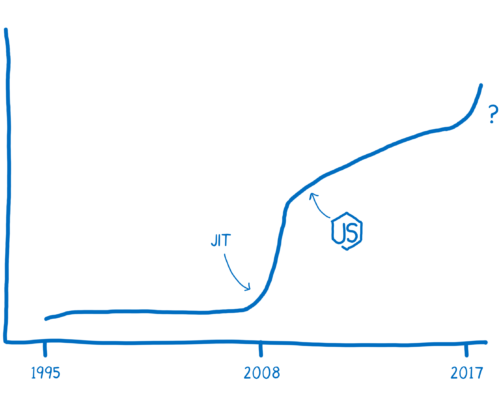
\includegraphics[width=0.7\textwidth,height=0.7\textheight]{./images/perf_history.png}
        \caption{\href{https://hacks.mozilla.org/2017/02/a-cartoon-intro-to-webassembly/}{Performance on the Web}}
    \end{figure}
\end{frame}


\begin{frame}
    \setbeamerfont{subsection in toc}{size=\small}
    \frametitle{Agenda}
    \begin{multicols}{2}
    \tableofcontents
    \end{multicols}
\end{frame}

\section{Basics} 

\subsection{Definition}

\begin{frame}{Definition}
    \begin{figure}
        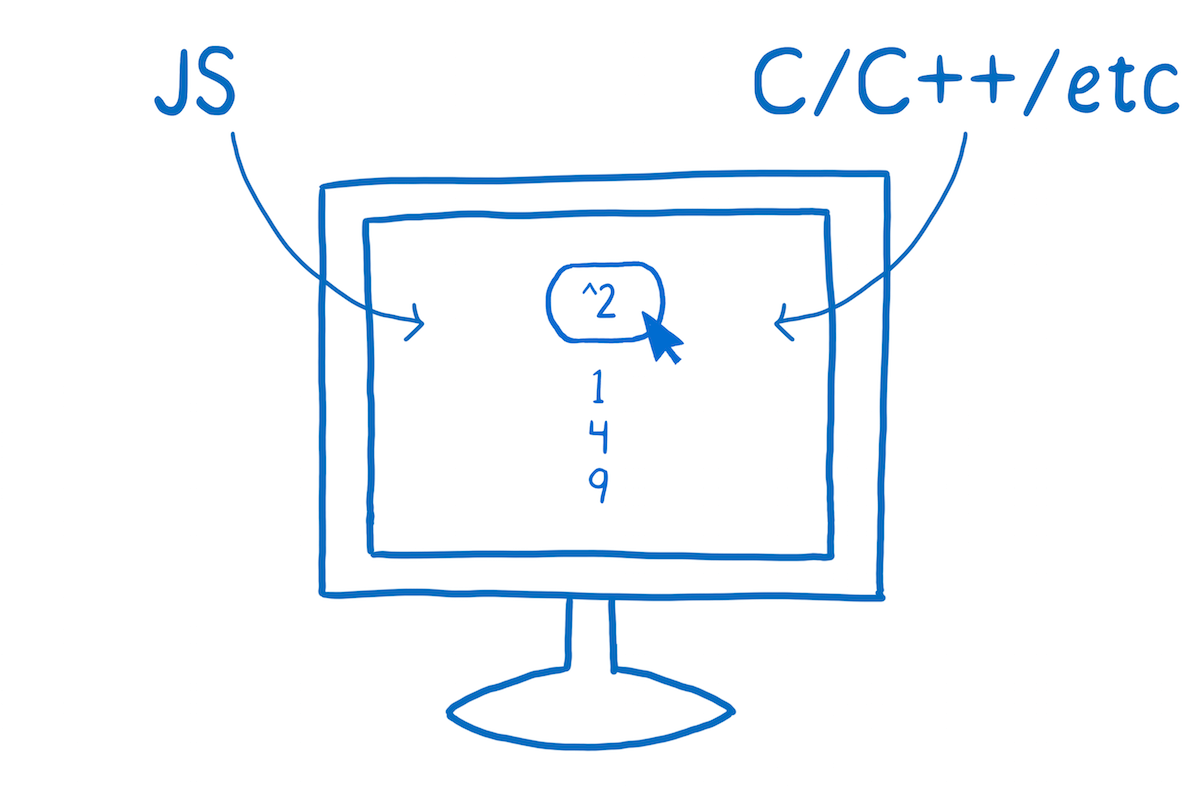
\includegraphics[scale=0.2]{./images/definition.png}
        \caption{\href{https://www.smashingmagazine.com/2017/05/abridged-cartoon-introduction-webassembly/}{Introduction to WebAssembly}}
    \end{figure}
\end{frame}

\begin{frame}{Definition}
    \begin{figure}
        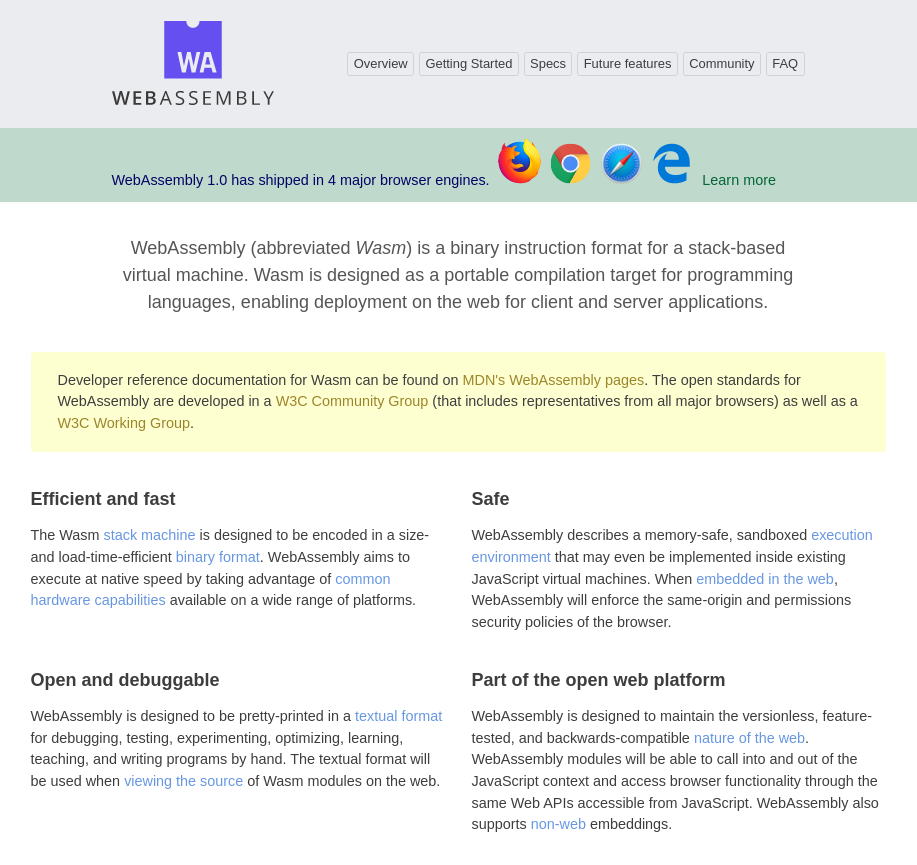
\includegraphics[scale=0.2]{./images/webassembly_org.png}
        \caption{\href{https://webassembly.org/}{webassembly.org}}
    \end{figure}
\end{frame}

\begin{frame}{Definition}
    \begin{quotation}
        "\textbf{WebAssembly} (abbreviated Wasm) is a \textbf{binary instruction format} for a \textbf{stack-based virtual machine}. Wasm is designed as a \textbf{portable compilation target} for programming languages, \textbf{enabling deployment on the web} for client and server applications."
    \end{quotation}
\end{frame}

\subsection{Key Concepts}

\begin{frame}{Binary Instruction Format}
    \begin{itemize}
        \item \textbf{Machine code} $||$ \textbf{Bytecode for a virtual machine}
        \item \textbf{Targeting different instruction set architectures} (ISA) like \textbf{x86}, \textbf{ARM} or \textbf{RISC-V}
        \item WASM uses \textbf{virtual instructions} for a \textbf{conceptual machine}, not a physical one
        \item Think of WASM instruction set as \textbf{intersection of multiple ISAs} that can't be mapped directly to one ISA
    \end{itemize}
\end{frame}

\begin{frame}{Stack-Based Virtual Machine}
    \begin{itemize}
        \item Virtual machine which \textbf{uses stack} data structure \textbf{to perform operations}
        \item Famous stack-based VMs are the \textbf{JVM} (Java Virtual Machine) and the \textbf{CLR} (Common Language Runtime)
        \item When the \textbf{browser} translates WASM to the machine code for the machine the browser is running on, it \textbf{will use registers}. Since the WASM specification does \textbf{not} specify registers, it gives the browser more \textbf{flexibility} to use the \textbf{best register allocation} for  that machine
    \end{itemize}
\end{frame}

\begin{frame}{Portable Compilation Target}
    \begin{itemize}
        \item \textbf{WASM is designed to be executable on a variety of operating systems and instruction set architectures, on the Web and off the Web}
        \item \textbf{Low requirements} for WASM execution environments:
              \begin{itemize}
                  \item 8-bit Bytes
                  \item Addressable at byte granularity
                  \item Little endian
                  \item \href{https://webassembly.org/docs/portability/}{...}
              \end{itemize}
    \end{itemize}
\end{frame}

\begin{frame}{Deployment on the Web Platform}
    \begin{itemize}
        \item The \textbf{web platform} can be described in two parts
              \begin{itemize}
                  \item A \textbf{VM/Engine} that runs the code, e.g. V8 or SpiderMonkey
                  \item A set of \textbf{Web APIs} that can be called to control browser/device functionality (DOM, WebGL, Web Audio API etc.)
              \end{itemize}
        \item The VM can now load an run two types of code: \textbf{JavaScript and WebAssembly}
        \item V8 using \textbf{Liftoff} as one-pass WASM compiler and \textbf{TurboFan} for optimizations
        \item As of Dec. 2021, \textbf{95\%} of all installed browsers support WASM.
        \item The different code types \textbf{can call each other}
    \end{itemize}
\end{frame}

\begin{frame}{Definition}
    \begin{quotation}
        "\textbf{WebAssembly} (abbreviated Wasm) is a \textbf{binary instruction format} for a \textbf{stack-based virtual machine}. Wasm is designed as a \textbf{portable compilation target} for programming languages, \textbf{enabling deployment on the web} for client and server applications."
    \end{quotation}
\end{frame}

\subsection{Use Cases}

\begin{frame}{Use Cases}
    \textbf{Inside of the Browser:}
    \begin{itemize}
        \item \textbf{VR} and \textbf{AR}
        \item \textbf{Simulation}/\textbf{Emulation} (DOSBox, QEMU, …)
        \item \textbf{Remote desktop}
        \item \textbf{Games}
        \item \textbf{Cloud IDEs}
        \item \href{https://webassembly.org/docs/use-cases/}{...}
    \end{itemize}
    \textbf{Outside of the browser:}
    \begin{itemize}
        \item \textbf{Server-side applications}
        \item Game \textbf{distribution} services
    \end{itemize}
\end{frame}

\begin{frame}{Projects using WebAssembly}
    \begin{itemize}
        \item \textbf{Blazor}
        \item \textbf{AutoCAD}
        \item \textbf{Figma}
        \item \textbf{Jitsi} for virtual backgrounds
        \item \textbf{Zoom} for video encoding
        \item \textbf{\href{https://wasm.continuation-labs.com/d3demo/}{D3wasm}}
        \item \textbf{go-app}/\textbf{yew}
        \item ...
    \end{itemize}
\end{frame}

\subsection{WebAssembly Text}

\begin{frame}[fragile]{WebAssembly Text}
    \begin{itemize}
        \item \textbf{Textual representation} of the binary format to allow reading and editing by humans
        \item Designed to be \textbf{exposed} in \textbf{text editors}, \textbf{browser developer tools}, etc.
        \item Files can be compiled to using the \textbf{WebAssembly Binary Toolkit} (WABT)
        \item For more information, consider visiting the \textbf{\href{https://developer.mozilla.org/en-US/docs/WebAssembly/Understanding_the_text_format}{MDN Web Docs}}
    \end{itemize}
\end{frame}

\begin{frame}{WebAssembly Text - Example}
    \begin{figure}
        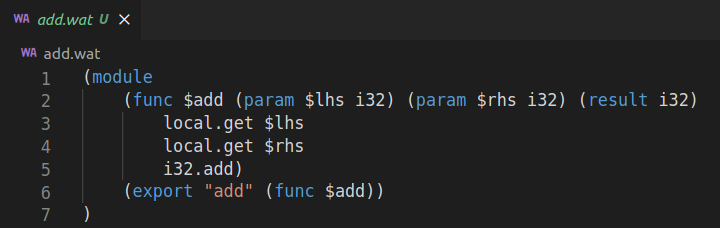
\includegraphics[scale=0.3]{./images/wat.png}
        \caption{WebAssembly Module with a simple add function}
    \end{figure}
    \begin{figure}
        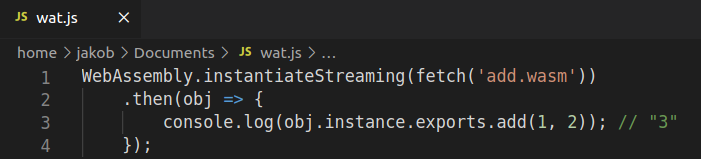
\includegraphics[scale=0.3]{./images/watjs.png}
        \caption{Calling the function}
    \end{figure}
\end{frame}

\section{Demo}

\begin{frame}{Demo - Prerequisites}
    \textbf{Disclaimer}
    \begin{itemize}
        \item This demo is using the \textbf{\href{https://go.dev/}{Go}} programming language. You don't need any knowledge about Go to follow this demo. Furthermore, I am using \textbf{Linux}! I can't guarantee, nor do I care, that it works on your Windows machine.
    \end{itemize}
    \textbf{Installing Go}
    \begin{itemize}
        \item Please follow \underline{\href{https://go.dev/doc/install}{this}} tutorial
    \end{itemize}
\end{frame}

\subsection{Supported Languages}

\begin{frame}{Supported Languages}
    \begin{figure}
        
\includegraphics[scale=0.3]{./images/langs.png}
        \caption{Production Ready Languages}
    \end{figure}
\end{frame}


\subsection{Hello World}

\begin{frame}{Demo - File structure}
    \begin{figure}
        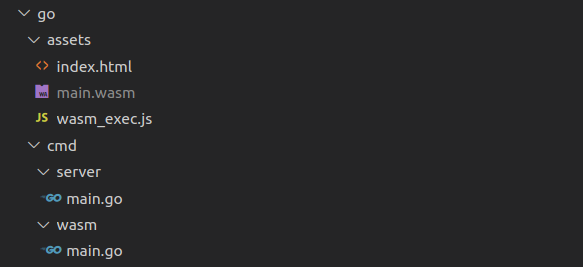
\includegraphics[scale=0.5]{./images/structure.png}
        \caption{File structure}
    \end{figure}
\end{frame}


\begin{frame}{Demo - cmd/wasm/main.go}
    \begin{figure}
        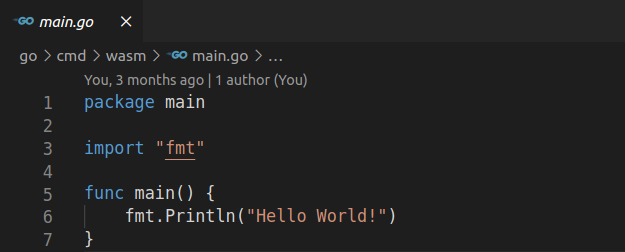
\includegraphics[scale=0.5]{./images/main2.png}
        \caption{main.go}
    \end{figure}
\end{frame}

\begin{frame}[fragile]{Demo - Compilation}
    \begin{itemize}
    \item To compile your main.go to a WebAssembly main.wasm file, \textbf{execute} the following command in the wasm directory:
    \begin{lstlisting}[language=Bash,basicstyle=\scriptsize]
GOOS=js GOARCH=wasm go build -o  ../../assets/main.wasm
    \end{lstlisting}
    
    \item You should now be able to locate a \lstinline{main.wasm} file inside your \lstinline{assets} folder.
\end{itemize}
\end{frame}

\begin{frame}[fragile]{Demo - JavaScript Glue Code}
    \begin{itemize}
    \item Some JavaScript code is needed to import the WebAssembly Module we just created in the Browser. Fortunately, this code comes with every Go installation. So just go ahead and copy the file into your \lstinline{assets} directory:

    \begin{lstlisting}[language=Bash,basicstyle=\scriptsize]
cp "$(go env GOROOT)/misc/wasm/wasm_exec.js" .
\end{lstlisting}
\end{itemize}
\end{frame}

\begin{frame}{Demo - assets/index.html}
    \begin{figure}
        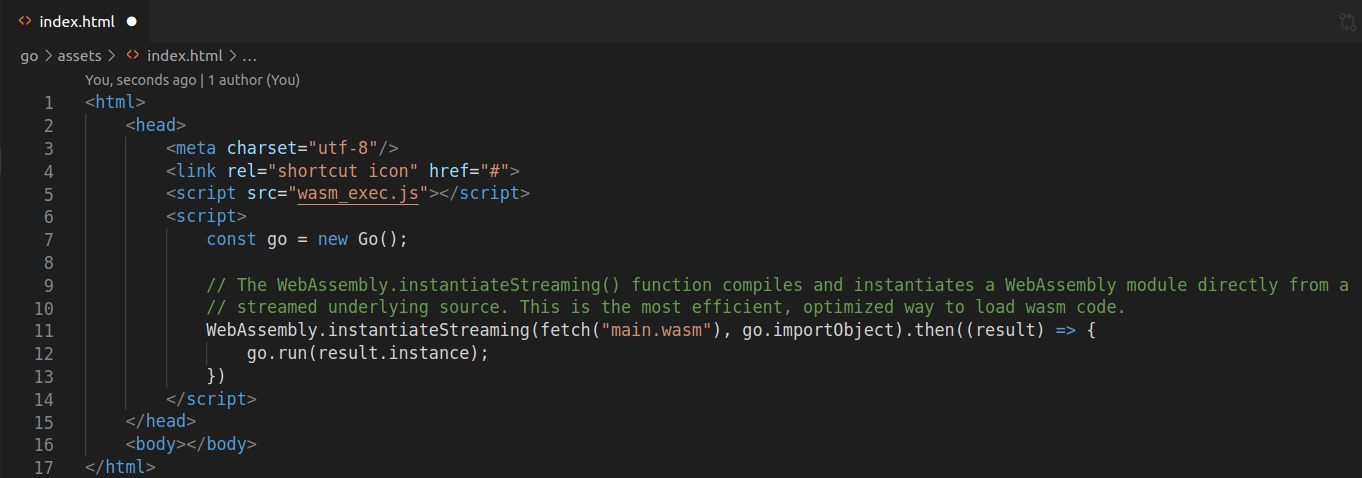
\includegraphics[scale=0.2]{./images/idx.png}
        \caption{index.html}
    \end{figure}
\end{frame}

\begin{frame}{Demo - cmd/server/main.go}
    \begin{figure}
        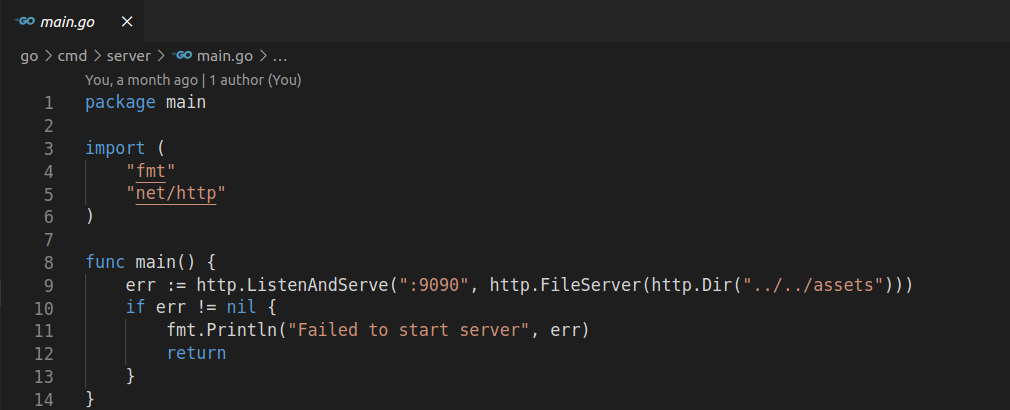
\includegraphics[scale=0.3]{./images/server.png}
        \caption{main.go}
    \end{figure}
\end{frame}

% Show resulting wasm file and code in the browser
% Show rust demo as well - cargo install wasm-pack, wasm-pack build --target web
\begin{frame}[fragile]{Demo - Execution}
    \begin{itemize}
    \item  Now you can run your server and inspect the outcome. Make sure you are in the \lstinline{server} directory, when executing this command:
    \begin{lstlisting}[language=bash,basicstyle=\scriptsize]
 go run main.go
\end{lstlisting}

    \item Now you should be able to inspect the result in your browser:
    \begin{figure}
        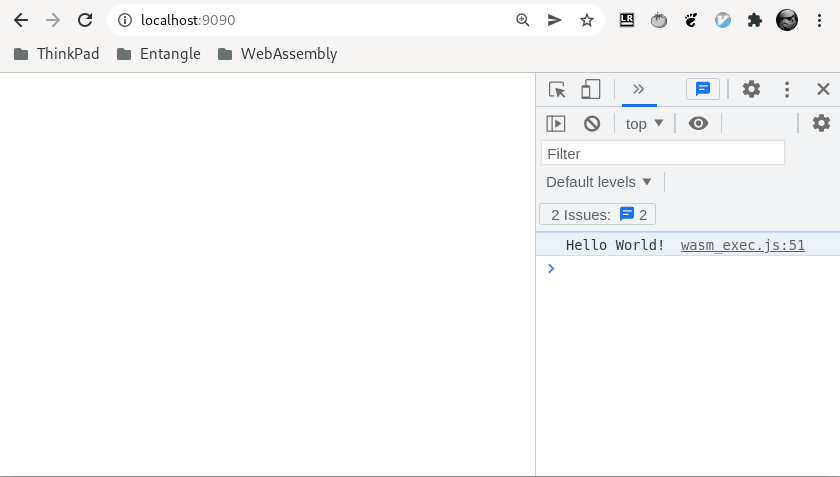
\includegraphics[scale=0.2]{./images/demo.png}
        \caption{\href{https://hacks.mozilla.org/2017/02/a-cartoon-intro-to-webassembly/}{Performance-Entwicklung im Web-Kontext}}
    \end{figure}
    \end{itemize}
\end{frame}

\subsection{Exports}

\begin{frame}{Demo - Exports}
    \begin{figure}
        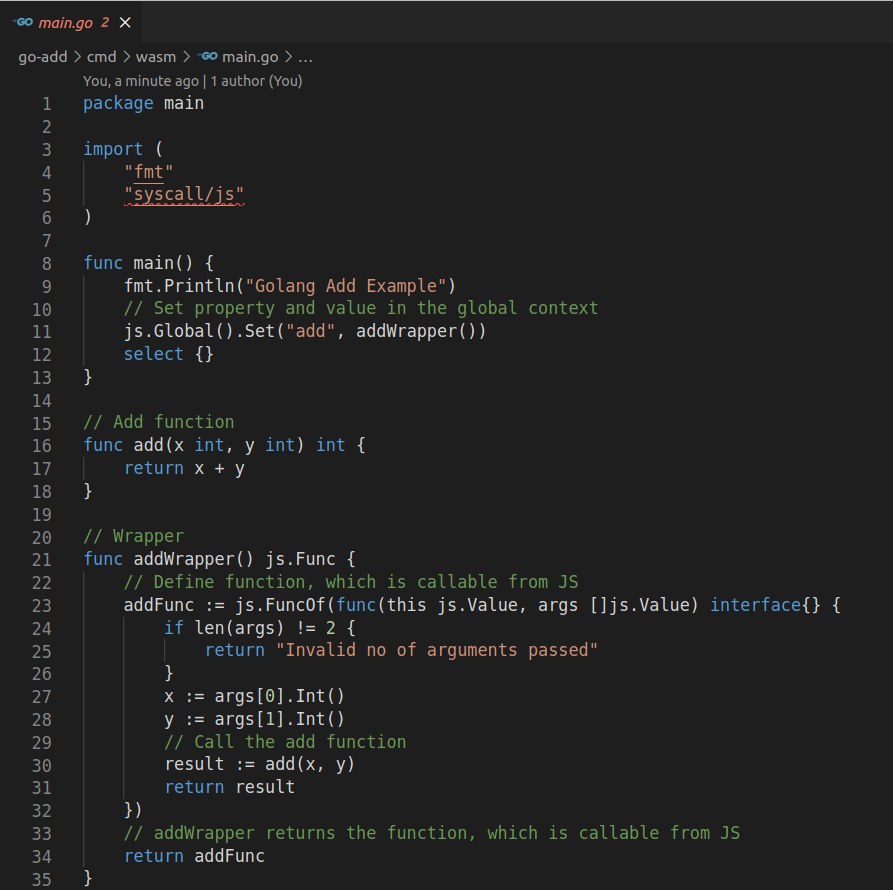
\includegraphics[scale=0.2]{./images/goaddmain.png}
        \caption{cmd/wasm/main.go}
    \end{figure}
\end{frame}

\begin{frame}{Demo - Exports}
    \begin{figure}
        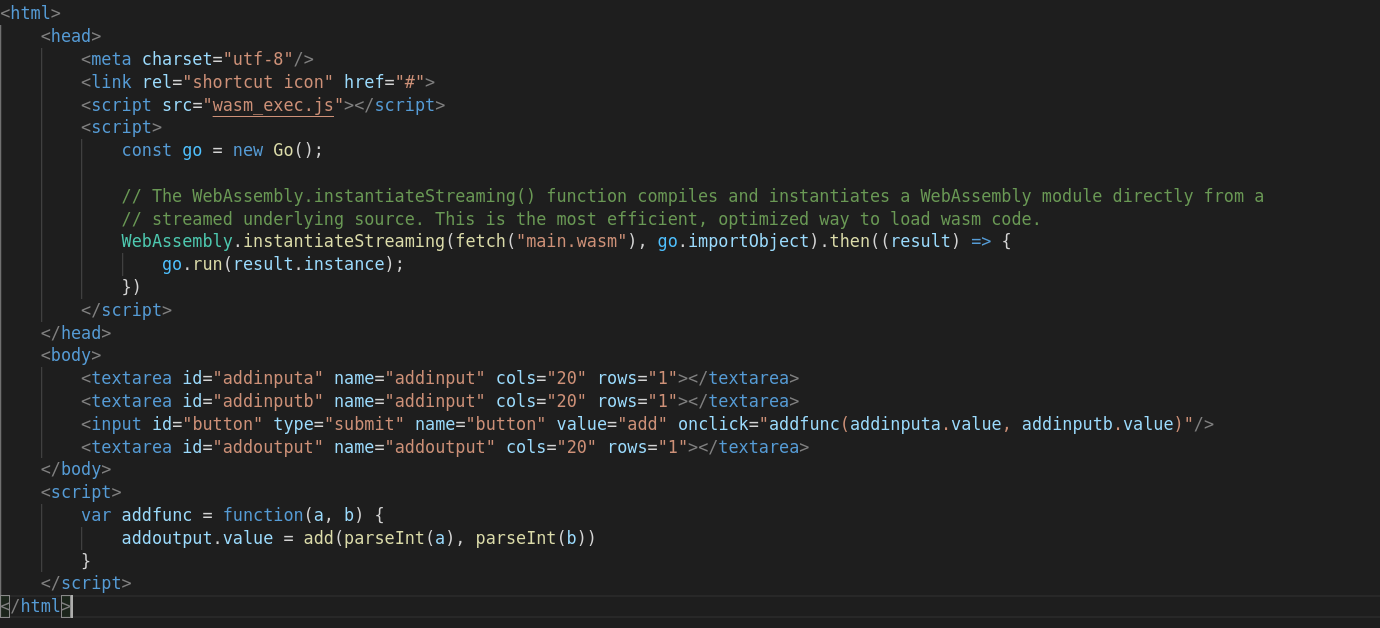
\includegraphics[scale=0.2]{./images/index.png}
        \caption{assets/index.html}
    \end{figure}
\end{frame}

\subsection{Imports}

\begin{frame}{Demo - Imports}
\begin{figure}
        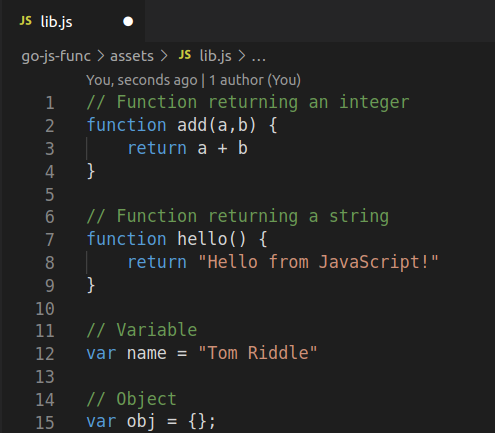
\includegraphics[scale=0.4]{./images/libjsfunc.png}
        \caption{assets/lib.js}
    \end{figure}
\end{frame}

\begin{frame}{Demo - Imports}
 \begin{figure}
        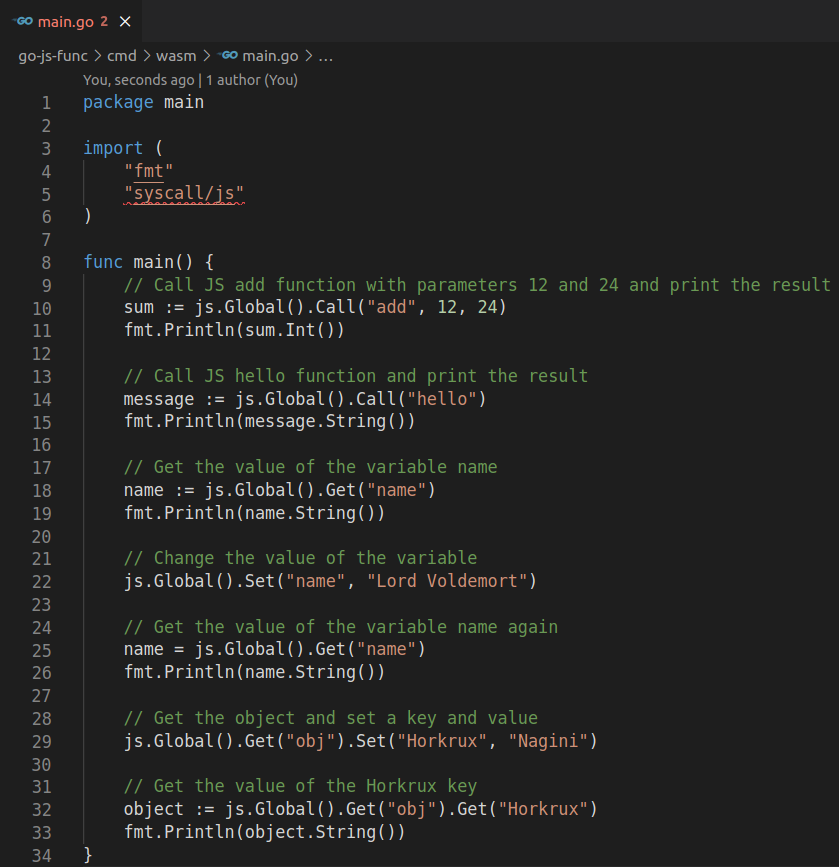
\includegraphics[scale=0.2]{./images/jsfuncmain.png}
        \caption{cmd/wasm/main.go}
    \end{figure}
\end{frame}

\begin{frame}{Demo - Imports}
    \begin{figure}
        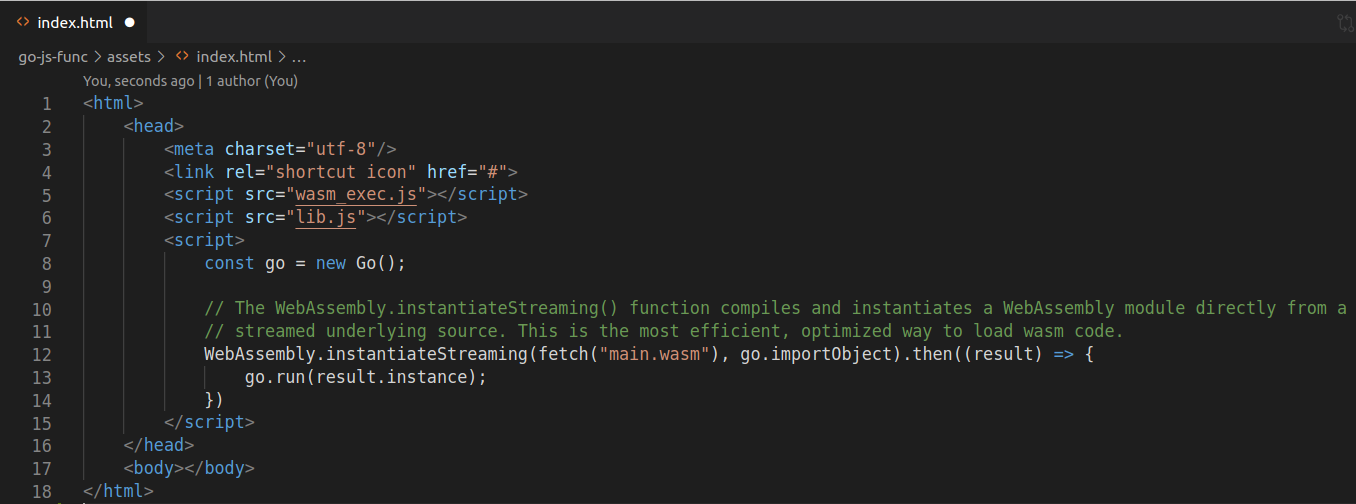
\includegraphics[scale=0.2]{./images/importindex.png}
        \caption{assets/index.html}
    \end{figure}
\end{frame}

\begin{frame}{Additional Information}
    \begin{itemize}
        \item WebAssembly functions only support \textbf{integers} and \textbf{floating point numbers}. To work with other data types, linear memory can be used
        \item \textbf{Linear Memory} - Continuous buffer of unsigned bytes that can be read from and stored into by both Wasm and Javascript
        \item \textbf{No DOM Manipulation} - Use JS with e.g. \textbf{syscall/js} in \textbf{Go} or \textbf{wasm-bindgen} in \textbf{Rust}. \textbf{AssemblyScript} provides those features out of the box...
        \item \textbf{Multithreading} utilizing Web Workers
    \end{itemize}
\end{frame}

\begin{frame}{Terminology}
    \begin{itemize}
        \item \textbf{Module}: WebAssembly Binary that has beed compiled into executable machine code. A Module is stateless and thus, like a Blob, can be explicitly shared between windows and workers.
        \item \textbf{Memory}: A resizable ArrayBuffer that contains the linear array of bytes which can be used from WebAssembly and JavaScript 
        \item \textbf{Table}: A resizable typed array of references (e.g. to functions) that could not otherwise be stored as raw bytes in Memory. 
        \item \textbf{Instance}:  A Module paired with Memory, Table and Imports.
    \end{itemize}
\end{frame}


% Lucet is deprecated for wasmtime
% Add a bit more theory
\section{Advanced Concepts}

\subsection{WebAssembly Runtimes}

\begin{frame}{WebAssembly Runtimes}
    \begin{itemize}
        \item \textbf{Run WebAssembly outside of the browser}
        \item \textbf{Wasmer} - lightweight containers that run everywhere
        \item \textbf{Wasmtime} - standalone JIT style runtime based on cranelift
        \item \textbf{WebAssembly Micro Runtime} (WAMR)
    \end{itemize}
\end{frame}

\subsection{WebAssembly System Interface}

\begin{frame}{WebAssembly System Interface - WASI}
\begin{itemize} 
    \item \textbf{Interact with system} using syscalls
    \item Normally, the \textbf{standard library} of a programming language \textbf{provides} said \textbf{system interface} which is os-dependent
    \item E.g. \lstinline{prinft} being compiled for a Windows machine could use the \textbf{Windows API} to interact with the machine. If it's being compiled for Mac or Linux, \textbf{POSIX} will be used
    \item With WASM you \textbf{don't know which operating system} you're targeting even when you're compiling. So you can't use any single OS system interface 
    \item WASI provides a \textbf{compatible implementation} with multiple OSs
    \item Portability and Security with \textbf{Sandboxing}
\end{itemize}
\end{frame}

\subsection{WebAssembly Gateway Interface}
\begin{frame}{WebAssembly Gateway Interface - WAGI*}
    \begin{itemize}
        \item Write \textbf{microservices} and \textbf{web apps}
        \item Run WASM binaries as \textbf{HTTP handlers} using \textbf{STDIN} and \textbf{STDOUT} and \textbf{environment variables}
        \item When HTTP \textbf{request} is received the WASM binary gets executed with the necessary Information contained in STDIN and environment variables
        \item \textbf{Responses} are sent to STDOUT and binary can terminate again.
        \item \textbf{WAGI-Server} can be used
    \end{itemize}
\end{frame}


\section{Evaluation}

\begin{frame}{Evaluation}
    \begin{figure}
        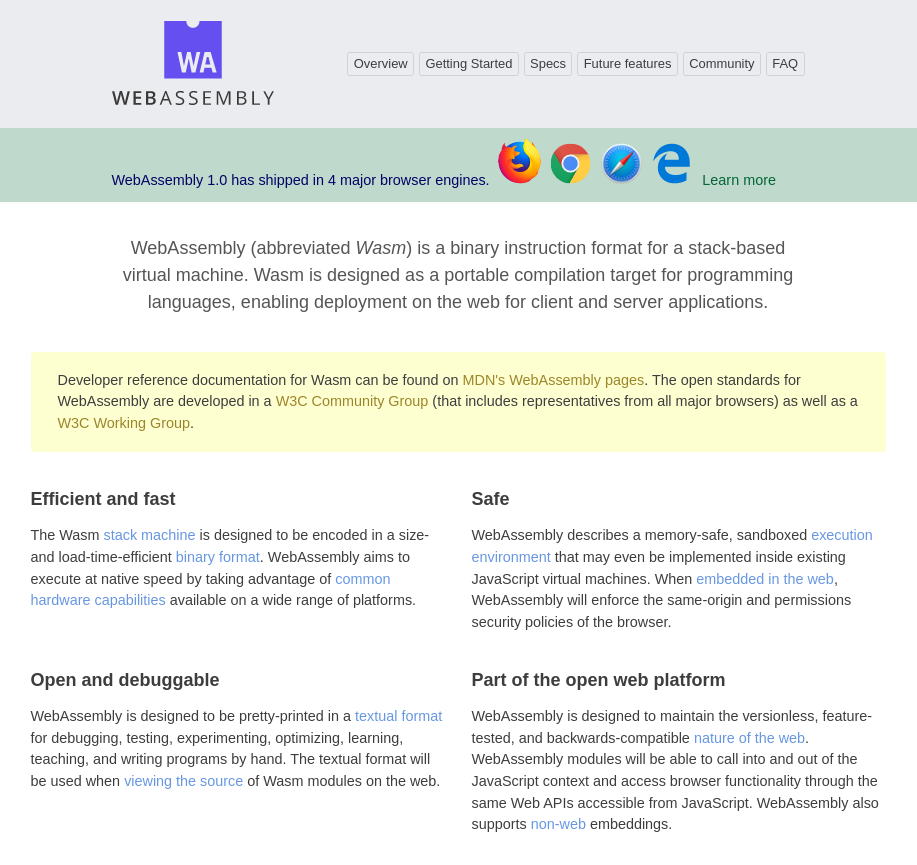
\includegraphics[scale=0.2]{./images/webassembly_org.png}
        \caption{\href{https://webassembly.org/}{webassembly.org}}
    \end{figure}
\end{frame}

\subsection{Efficient and Fast}

\begin{frame}{Efficient and fast}
    \begin{figure}
        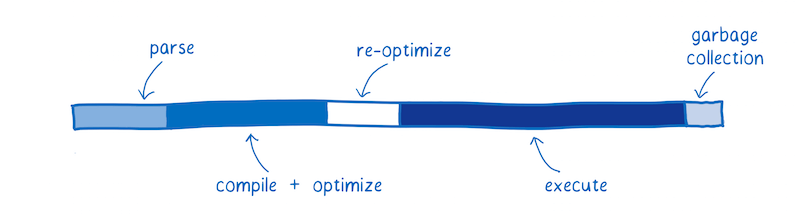
\includegraphics[scale=0.3]{./images/javascriptgraph.png}
        \caption{\href{https://www.smashingmagazine.com/2017/05/abridged-cartoon-introduction-webassembly/}{Time distribution when running JavaScript}}
    \end{figure}
    \begin{figure}
        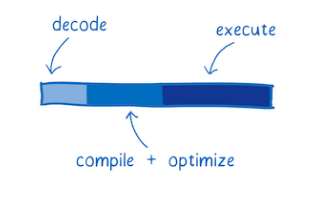
\includegraphics[scale=0.4]{./images/wasmgraph.png}
        \caption{\href{https://www.smashingmagazine.com/2017/05/abridged-cartoon-introduction-webassembly/}{Time distribution when running WebAssembly}}
    \end{figure}
\end{frame}

\begin{frame}{Efficient and fast - Compilation + Optimization}
    \begin{figure}
        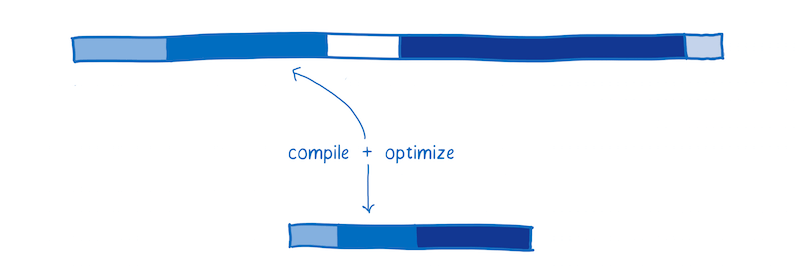
\includegraphics[scale=0.2]{./images/copyoptimize.png}
        \caption{\href{https://www.smashingmagazine.com/2017/05/abridged-cartoon-introduction-webassembly/}{Compilation}}
    \end{figure}
    \begin{itemize}
        \item JavaScript is \textbf{compiled during the execution} of the code
        \begin{itemize}
            \item Because types are \textbf{dynamic}, multiple versions of the same code may need to be compiled.
        \end{itemize}
        \item WebAssembly saves time with regards to:
              \begin{itemize}
                  \item Not needing to figure out \textbf{types}
                  \item Ahead of time \textbf{optimizations}
              \end{itemize}
    \end{itemize}
\end{frame}

\begin{frame}{Effecient and fast - Execution}
    \begin{figure}
        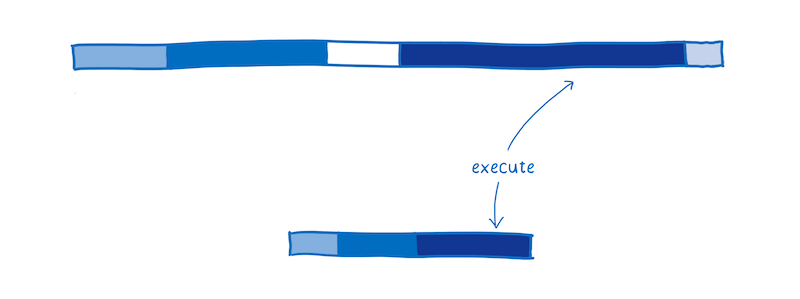
\includegraphics[scale=0.1]{./images/execution.png}
        \caption{\href{https://www.smashingmagazine.com/2017/05/abridged-cartoon-introduction-webassembly/}{Execution}}
    \end{figure}
    \begin{itemize}
        \item Most developers don't know about \textbf{JIT internals}, so writing performant JS code is hard
        \item WASM is \textbf{designed} to be a \textbf{compiler target}, not a human readable language. Instruction set is \textbf{optimized for machines}
        \item \textbf{Near native speed} (60-70\% in a C++ analysis). 
        \item \textbf{Causes} for decreased speed compared to native execution:
        \begin{itemize}
            \item Poor register allocation
            \item Reserved registers
            \item Poor instruction selection
            \item Stack overflow checks
        \end{itemize}
        \item \textbf{Still up to 800\% faster than JavaScript}
    \end{itemize}
\end{frame}


\begin{frame}{Evaluation}
    \begin{figure}
        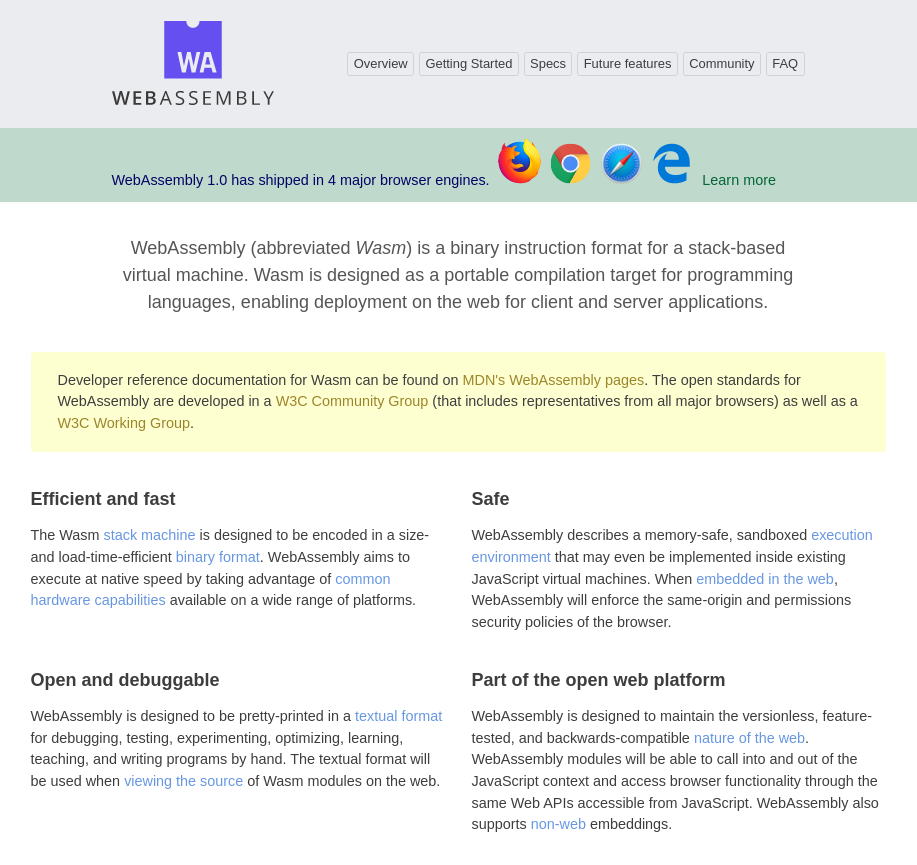
\includegraphics[scale=0.2]{./images/webassembly_org.png}
        \caption{\href{https://webassembly.org/}{webassembly.org}}
    \end{figure}
\end{frame}

\subsection{Security}

\begin{frame}{Security}
    \begin{itemize}
    \item \textbf{Sandboxing}
    \item \textbf{Same-Origin-Policy}
    \item \textbf{Permissions} are required to access hardware of filesystem
    \item \textbf{Dedicated memory space}
    \item \textbf{Prohibit unwanted memory access}
    \item \textbf{Protect execution stack}
    \item \textbf{Tables}
    \item \textbf{Traps}
    \end{itemize}
\end{frame}


\section{Conclusion}

\begin{frame}{Conclusion}
\begin{itemize}
    \item \textbf{Don't use it} for your website!
    \item \textbf{Do use it} for performance intensive tasks (AR, VR...)
    \item \textbf{Portability} and interoperability
    \item \textbf{Here to stay}
    \begin{itemize}
        \item Backed by the \textbf{Bytecode Allegiance} (ARM, Google, Intel, Microsoft, Mozilla...)
        \item \textbf{Krustlet} - Running WASM Modules instead of container images on K8s clusters
    \end{itemize}
\end{itemize}
\end{frame}

\begin{frame}{Conclusion}
    \begin{figure}
        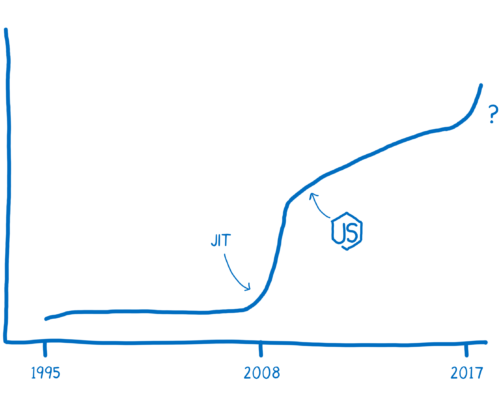
\includegraphics[width=0.7\textwidth,height=0.7\textheight]{./images/perf_history.png}
        \caption{\href{https://hacks.mozilla.org/2017/02/a-cartoon-intro-to-webassembly/}{Performance-Entwicklung im Web-Kontext}}
    \end{figure}
\end{frame}

\section{Webshop}

\begin{frame}{Webshop}
\end{frame}

\begin{frame}[fragile]{Sources}
    \begin{lstlisting}[language=Lisp,basicstyle=\tiny]
    https://developer.mozilla.org/en-US/docs/WebAssembly/Understanding_the_text_format
    https://webassembly.org/docs/portability/
    https://webassembly.org/docs/use-cases/
    https://radu-matei.com/blog/practical-guide-to-wasm-memory/
    https://www.smashingmagazine.com/2017/05/abridged-cartoon-introduction-webassembly/
    https://hacks.mozilla.org/2017/02/what-makes-webassembly-fast/
    https://hacks.mozilla.org/2017/02/creating-and-working-with-webassembly-modules/
    https://github.com/golang/go/wiki/WebAssembly#getting-started
    https://golangbot.com/webassembly-using-go/
    https://madewithwebassembly.com/about/
    https://medium.com/@atilafassina/es2015-modules-101-d9977dc4d4c7
    https://developer.mozilla.org/en-US/docs/WebAssembly
    https://golangbot.com/go-webassembly-dom-access/
    https://wasmbyexample.dev/examples/exports/exports.go.en-us.html
    https://github.com/WebAssembly/design/issues/219
    https://hacks.mozilla.org/2018/10/calls-between-javascript-and-webassembly-are
    -finally-fast-\%f0\%9f\%8e\%89/
    https://www.infoq.com/podcasts/web-assembly-component-model/
    https://hacks.mozilla.org/2019/03/standardizing-wasi-a-
    webassembly-system-interface/
    https://webassembly.org/docs/web/
    https://webassembly.org/docs/security/
    https://www.virusbulletin.com/virusbulletin/2018/10/dark-side-webassembly/
    https://www.infoworld.com/article/3632865/understanding-wagi-the-
    webassembly-gateway-interface.html
    https://radu-matei.com/blog/intro-wasm-components/
    https://www.usenix.org/conference/atc19/presentation/jangda
    https://entwickler.de/security/webassembly-ist-das-sicher-oder-kann-das-weg/
    https://www.toomanybees.com/storytime/gluing-the-web-and-webassembly-together
    \end{lstlisting}
\end{frame}
\end{document}